\chapter{Methodology} % Main chapter title

\label{Chapter3}

\section{Choice: EDSR vs. CinCGAN}

At the start of this master thesis project my advisor gave me two papers as good state of the art methods that would do nicely EDSR (\cite{EDSR}) and CinCGAN (\cite{CinCGAN}) offer fundamentally different approaches to Super Resolution:

\hfill

EDSR builds on SRResNet (\cite{SRGAN}), which is an adaptation of ResNet (\cite{ResNet}) for SISR, removing Batch Normalization layers, thus reducing the computational and memory burden of the network on hardware and allowing for a deeper architecture and more complex non-linear model to be learned for LR/HR mapping. 

\hfill

CinCGAN uses CycleGAN's (\cite{CycleGAN}) idea of image to image translation to create an unsupervised model that can denoise and upsample images without training with LR/HR pairs by first denoising the input in LR space, and then upscaling it with a state of the art SISR model, in this case EDSR.

\hfill

While CinCGAN achieves performance comparable to SRGAN, I personally find CinCGAN's results visually un-appealing since it seems to introduce artifacts of its own.

\hfill

\begin{figure}[H]
\centering
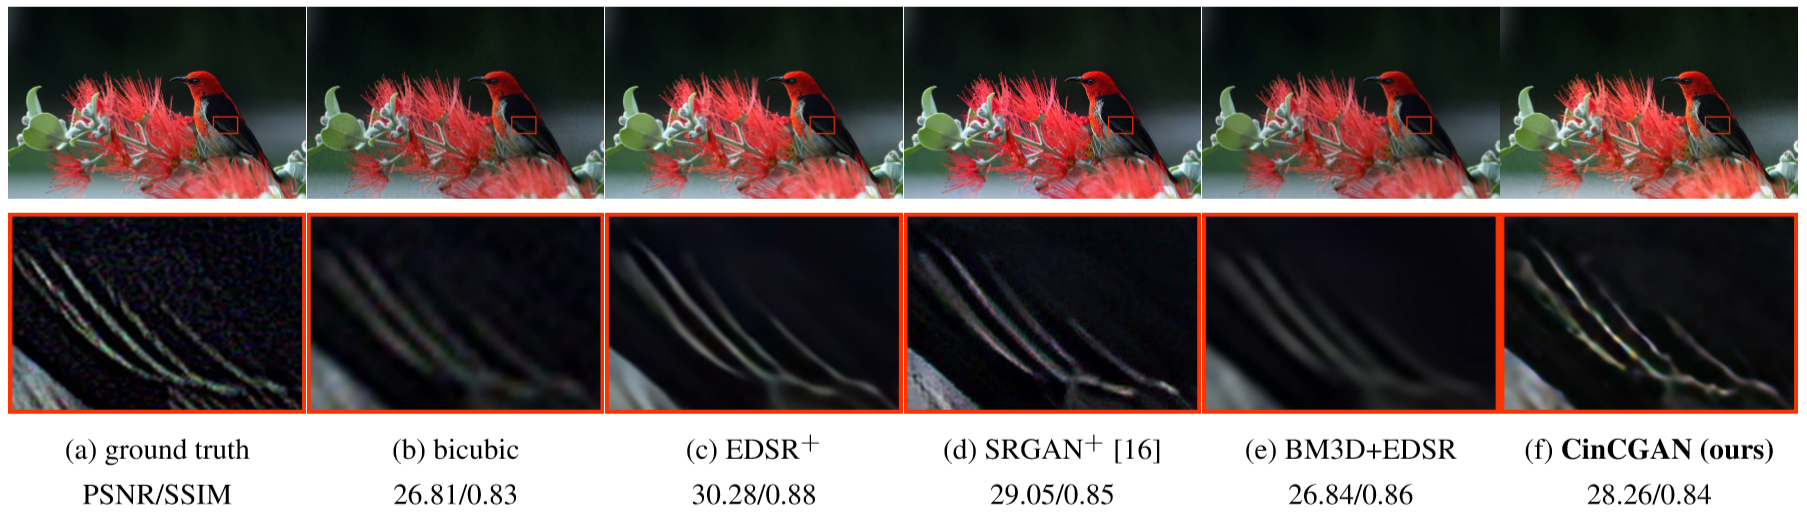
\includegraphics[width=\textwidth]{../Figures/CinCGAN2}
\caption{While SRGAN+'s result is not as sharp as the ground truth or CinCGAN's result, the lines in the latter case look distorted (Taken from the CinCGAN paper)}
\end{figure}

\begin{figure}[H]
\centering
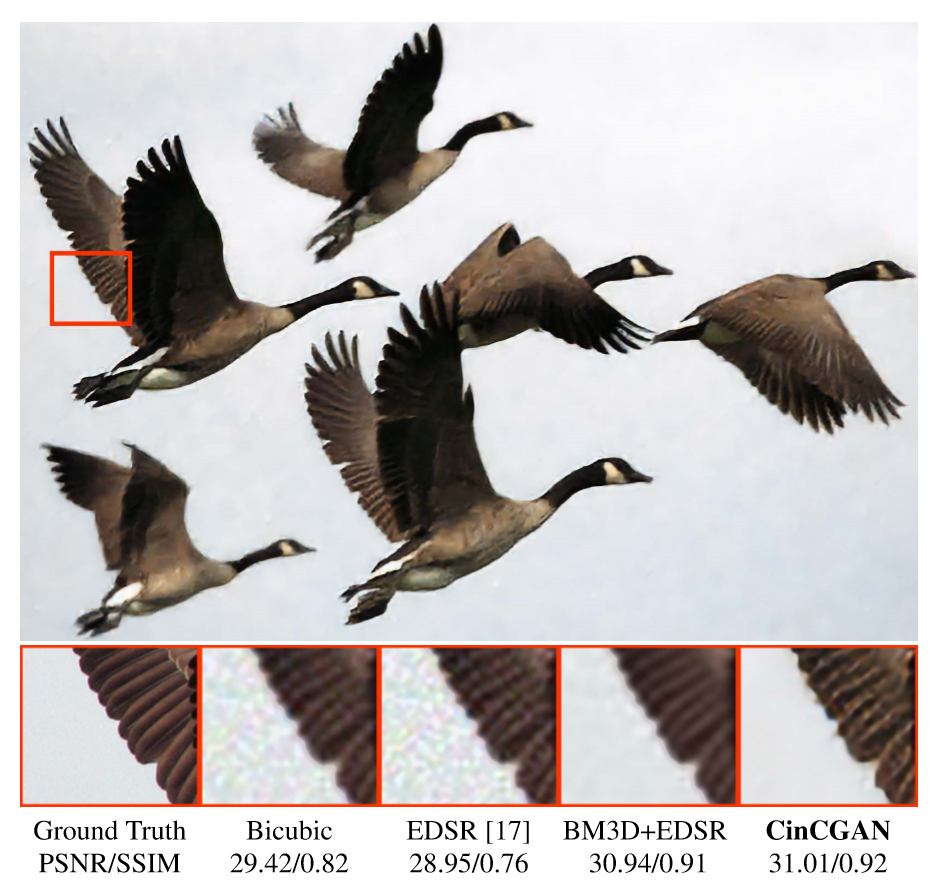
\includegraphics[width=0.75\textwidth]{../Figures/CinCGAN1}
\caption{While Bicubic and EDSR models can't denoise the image and BM3D+EDSR's result looks soft and blurry, the CinCGAN seems to introduce its own noise (Taken from the CinCGAN paper)}
\end{figure}

Since EDSR already performed the SR task inside CinCGAN and I didn't like the visual quality of the results given by the latter I chose to work with EDSR as a SR method, and would later think of a way of performing denoising.

\section{Choice: Denoising}

Denoising is a much more established and "stable" field, so when faced with the need to choose a denoising method I chose to look for extensively cited papers first instead of prioritizing state-of-the-art brand new ones.

\hfill

DnCNN (\cite{DnCNN}) is a residual neural network capable of handling gaussian noise and JPEG compression, its architecture according to the authors is a modified VGG (\cite{VGG}) network, adapting it for denoising instead of image recognition and implementing residual learning (\cite{ResNet}), the result is strikingly similar to SRResNet, and therefore, to EDSR, although SR tasks in DnCNN are performed by upscaling a LR image to HR size using bicubic interpolation and feeding it to the network.

\hfill

The way training data is created for DnCNN is to create patches with noise in the ranges of [0,55]$\sigma$ for gaussian noise and [5,99] quality for JPEG deblocking.

\hfill

I hypothesized that I could take the training method in DnCNN and use it with the EDSR architecture, since the only major differences were the lack of Batch Normalization layers, and the deconvolution and transpose process at the very end of EDSR, making its output larger than its input.

\hfill

DnCNN had been tested without Batch Normalization and it was shown that with Adam (\cite{Adam}), the training and performance impact of not using BN layers was small, so that wouldn't be a significant issue.

\begin{figure}[H]
\centering
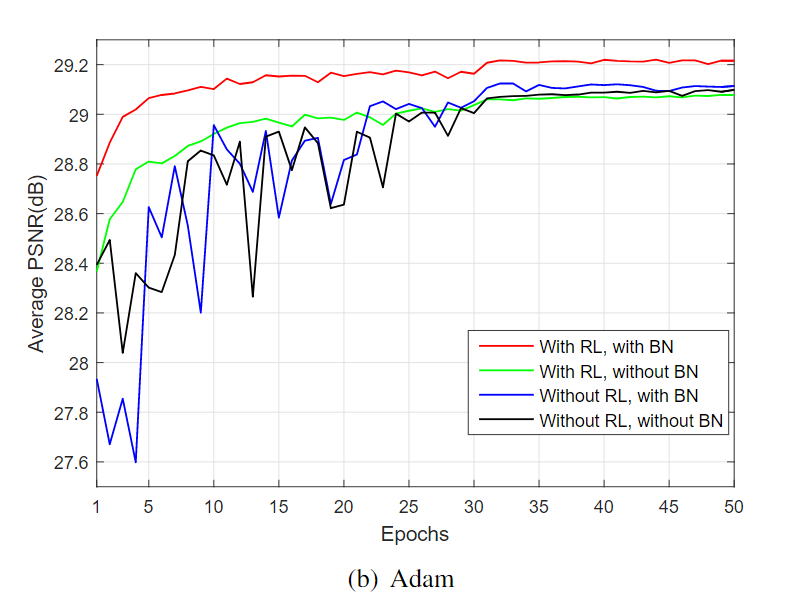
\includegraphics[width=0.75\textwidth]{../Figures/DnCNNAdam}
\caption{Impact of training DnCNN with and without BN (Taken from the DnCNN paper)}
\end{figure}

\section{Final decision}

I chose to use the EDSR architecture with a mixed training approach, the images in the training set would be split into overlapping patches, augmented with 90 degree rotations and then treated randomly in one of three ways (in all cases the HR patch is saved as a PNG intact):

\hfill

\begin{itemize}
    \item \textbf{Clean save}: the extracted patch would be downscaled using Lanczos resampling and saved as a PNG to preserve its quality.
    \item \textbf{JPEG save}: the extracted patch would be downscaled using Lanczos resampling and saved as a JPEG with a quality varying from 5 to 99.
    \item \textbf{Gauss save}: the extracted patch would be downscaled using Lanczos resampling, gaussian noise would be added to the patch with a standard deviation value between 0 and 55 and then saved as a PNG file.
\end{itemize}

\hfill

The network will follow the EDSR architecture and be trained with the Adam optimizer (learning rate: 1e-4, with it being halved every 200.000 updates, momentum: 0.9, variance momentum: 0.999, $\epsilon$: 1e-8) for 300.000 updates with a minibatch size of 16, for the loss function, L2 is used (as in SRResNet) instead of L1 (EDSR).

\begin{figure}[H]
\centering
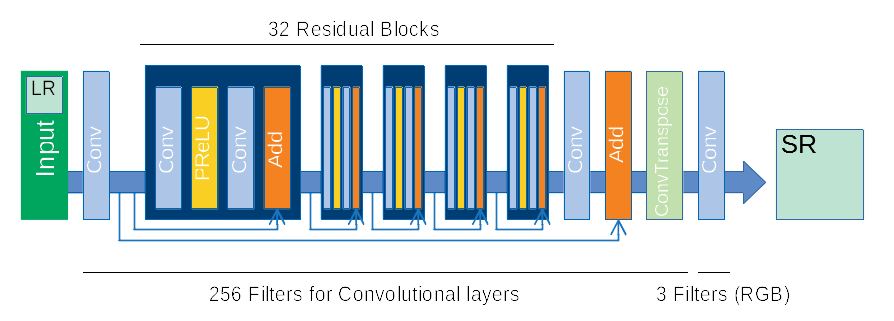
\includegraphics[width=0.75\textwidth]{../Figures/EDSR_Arch}
\caption{Implemented Architecture for 2x and 3x scales}
\end{figure}

\hfill

This for 4X upscaling has one more ConvolutionTranpose layer, this is especially useful for reusing the 2X model's weights to train a 4X model since the parameters of the layer remain the same.
